\chapter{Introduzione}

La \textbf{bioinformatica} nasce dall'incontro tra la biologia e le scienze computazionali e ha l'obiettivo di formalizzare problemi biochimici complessi e tradizionalmente legati all'osservazione sperimentale tramite automatizzazioni su larga scala. 

I sistemi biologici sono in grado di produrre dati come sequenque, strutture, reti di interazioni, eccetera\dots 
Questi, se opportunamente interpretati da sistemi informatici, possono rivelare le logiche molecolari alla base di processi come sistemi metabolici e la cura di malattie.

Questa disciplina è per sua natura \textbf{trasversale}. 
Un problema bioinformatico richiede simultaneamente 
la conoscenza della chimica per interpretare le 
proprietà molecolari, della biologia per comprendere 
il contesto cellulare e dell'informatica per 
costruire gli strumenti computazionali che rendano 
tutto ciò possibile su scale altrimenti inaccessibili 
all'indagine manuale. Si tratta quindi di sviluppare un linguaggio 
condiviso in cui le due discipline si integrano 
a vicenda.

Negli ultimi anni, l'\textbf{Intelligenza Artificiale} e il 
\textbf{Machine Learning} hanno cominciato a ridisegnare
questo ambito scientifico. Non come strumenti ausiliari di 
ottimizzazione, ma come motori di scoperta scientifica 
capaci di affrontare problemi che la ricerca tradizionale 
non aveva gli strumenti per risolvere. 

Un celebre caso particolarmente emblematico
di questo passaggio è \textbf{AlphaFold}, il sistema di 
predizione della struttura proteica sviluppato da DeepMind, 
che ha risolto in modo definitivo un problema aperto da oltre 
cinquant'anni, ovvero la predizione della conformazione 
tridimensionale di una proteina a partire dalla sua sola 
sequenza aminoacidica, e che è valso ai suoi sviluppatori 
il \textbf{Premio Nobel per la Chimica nel 2024} 
\cite{jumperHighlyAccurateProtein2021}.

\begin{figure}
    \centering
    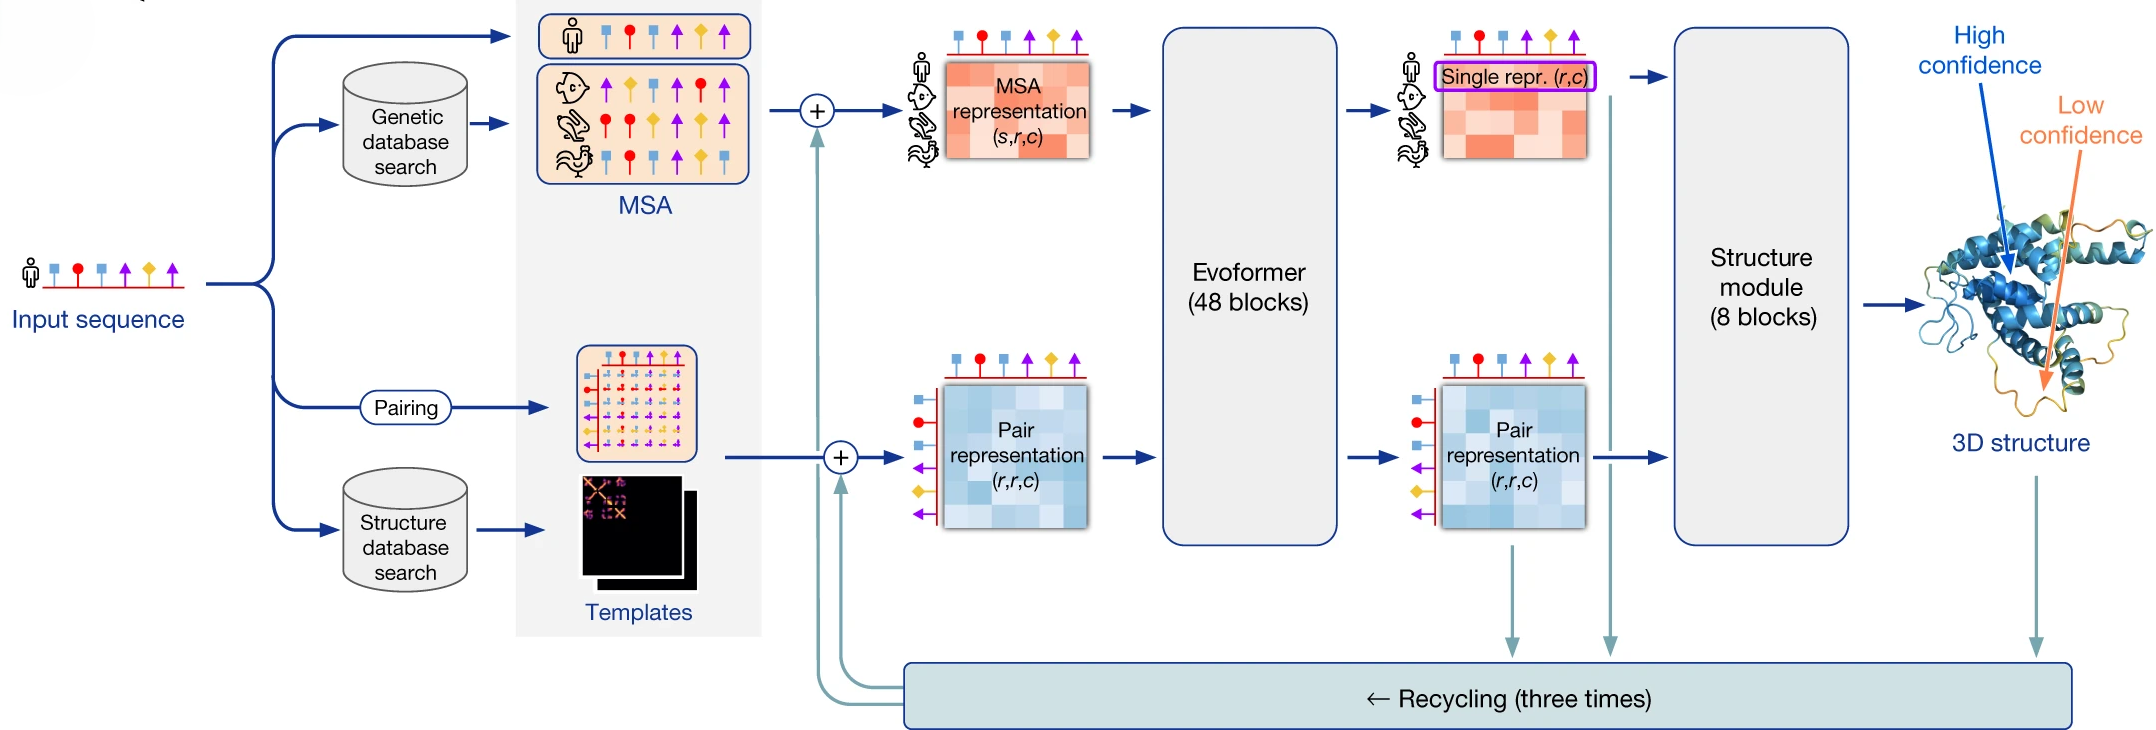
\includegraphics[width=1\linewidth]{figures/alphafold_pipeline.png}
    \caption{Schema semplificato della rete neurale di AlphaFold. Adattato e modificato dall'opera originale di Jumper et al. (2021), disponibile in Open Access sotto licenza Creative Commons Attribution 4.0 International (\url{http://creativecommons.org/licenses/by/4.0/}).}
    \label{fig:alphafold}
\end{figure}

Viene sfruttata un'architettura a rete neurale per integrare le nozioni chimico-fisiche e biologiche all'interno dell'insieme di regole di conformazione delle proteine.
Il modello si divide in due fasi principali:
\begin{enumerate}
    \item \textbf{Evoformer:} Primo modulo incaricato della previsione della struttura. Si approccia al problema computazionale interpretandolo come un \textbf{problema di inferenza di grafi} nello spazio tridimensionale. Tiene traccia degli amminoacidi propensi a mutare insieme, e a creare quindi strutture di avvolgimento complesse, tramite \textbf{Multiple Sequence Alignments} o \textbf{MSA}. Queste sono collezioni di sequenze di proteine omologhe allineate tra loro in un array bidimensionale, la cui analisi risulta utile per la previsone di coordinazioni tra amminoacidi e siti di ripiegamento proteico \cite{jumperHighlyAccurateProtein2021}.
    \item \textbf{Modello di Struttura:} Trasforma le informazioni ricavate dall'Evoformer in coordinate 3D reali. Ogni amminoacido è trattato come un corpo rigido indipendente, o "residue gas", che può ruotare e traslare nello spazio fino ad assumere la sua posizione "corretta" all'interno della conformazione della catena proteica.
    Viene usato un meccanismo di \textbf{Attenzione} (\textbf{Invariant Point Attentio, o IPA}) le cui iterazioni raffinano le informazioni spaziali degli elementi.
\end{enumerate}

AlphaFold non è un caso isolato. Nello stesso periodo, 
modelli di deep learning hanno identificato nuovi 
antibiotici attivi contro batteri resistenti 
\cite{stokesDeepLearningApproach2020}, permesso il 
"riposizionamento" di farmaci approvati durante 
la pandemia da COVID-19 \cite{richardsonBaricitinibPotentialTreatment2020}, 
e portato il primo farmaco interamente progettato da AI 
alla validazione clinica
\cite{xuGenerativeAIDiscoveredTNIK2025}. Questi risultati, 
che verranno discussi in dettaglio nel capitolo conclusivo, 
dimostrano come il ML applicato alla bioinformatica e in più particolare alla drug discovery sia già una realtà operativa nel campo della bioinformatica applicata alla \textit{drug discovery}.

\section{Obiettivi e Struttura dell'Elaborato}

Questo elaborato si propone di analizzare i principali 
metodi di Machine Learning e Deep Learning applicati 
alle fasi più critiche della pipeline farmaceutica, 
con particolare attenzione alla predizione delle 
interazioni farmaco-bersaglio e alla valutazione delle 
proprietà ADMET. 

La tesi studierà come la biologia molecolare e la farmacologia forniscano il 
contesto e il problema, mentre l'informatica (rappresentazione dei dati, architetture di apprendimento, 
ottimizzazione) fornisca gli strumenti e il linguaggio 
dell'analisi.

L'elaborato è organizzato come segue:

Il \textbf{Capitolo 2} introduce la pipeline di sviluppo 
farmaceutico, descrivendo le fasi principali del processo, dalla \textit{target identification} alla \textit{Lead Optimization} fino 
ai trial clinici, e il ruolo che l'AI svolge in ciascuna 
di esse. 
Vengono discussi l'attrition rate, il suo impatto 
economico e le cause principali del fallimento dei candidati 
farmaci.

Il \textbf{Capitolo 3} affronta il problema della 
rappresentazione molecolare, ovvero come tradurre entità 
biochimiche complesse, come molecole e proteine, in formati 
elaborabili da algoritmi di ML. 
Vengono analizzate le 
rappresentazioni lineari (SMILES, SELFIES), i fingerprint 
molecolari e le rappresentazioni a grafo.

Il \textbf{Capitolo 4} è il capitolo centrale dell'elaborato 
e tratta la predizione delle interazioni farmaco-bersaglio 
come problema computazionale formale. Dopo aver introdotto 
la formalizzazione matematica del problema DTI e DTA, 
vengono analizzate le metodologie di predizione, partendo dai 
metodi ligand-based e structure-based al docking 
molecolare, fino a trattare le architetture di Deep Learning 
più recenti: CNN, RNN, GNN e Transformer.

Il \textbf{Capitolo 5} tratta la valutazione delle 
proprietà ADMET, illustrando come il ML permetta di 
anticipare computazionalmente le cause più comuni di 
fallimento clinico, in particolare la tossicità molecolare, riducendo l'attrition rate 
nelle fasi avanzate della pipeline.
Verrà illustrata un'architettura multimodale d'esempio per ottimizzare la predizione e l'elaborazione delle conoscenze biochimiche, partendo dalle rappresentazioni dei farmaci candidati.

Il \textbf{Capitolo 6} presenta le conclusioni e 
sintetizza i contributi dei metodi analizzati,
documentando tre casi concreti di successo clinico (Baricitinib, Halicin e Rentosertib) che dimostrano il potenziale degli strumenti basati su AI 
nella drug discovery.